
\begin{table*}[t]
\centering
\setlength{\tabcolsep}{5pt}
\begin{tabular}{l | ccc | ccc | ccc}
\toprule
& \multicolumn{3}{c}{\textbf{First run, no retries}} 
& \multicolumn{3}{c}{\textbf{First run, w/ retries}} 
& \multicolumn{3}{c}{\textbf{Multiple runs, w/ retries}} \\
\cmidrule(lr){2-4} \cmidrule(lr){5-7} \cmidrule(lr){8-10}
\textbf{Model }
& \textit{base}$_{1,1}$ & \textit{ours}$_{1,1}$ & $\Delta$ 
& \textit{base}$_{1,5}$ & \textit{ours}$_{1,5}$ & $\Delta$ 
& \textit{base}$_{3,5}$ & \textit{ours}$_{3,5}$ & $\Delta$ \\
\midrule
o1 
& 10\% & \textbf{48\%} & +38\% 
& 38\% & \textbf{68\%} & +30\% 
& 52\% & \textbf{80\%} & +28\% \\

GPT-5 
& 44\% & \textbf{64\%} & +20\% 
& 80\% & \textbf{96\%} & +16\% 
& 88\% & \textbf{96\%} & +8\% \\

Gemini-Flash-2.5 
& 22\% & \textbf{48\%} & +26\% 
& 58\% & \textbf{74\%} & +16\% 
& 72\% & \textbf{86\%} & +14\% \\

Claude Sonnet-4.6 
& 28\% & \textbf{60\%} & +32\% 
& 58\% & \textbf{78\%} & +20\% 
& 78\% & \textbf{86\%} & +8\% \\
\bottomrule
\end{tabular}
\caption{Proof accuracy (\%) of the base model and our analogy-based method across settings. \textit{base}$_{i,j}$ denotes the base model with up to $i$ runs and $j$ retries, while \textit{ours}$_{i,j}$ denotes our method. $\Delta$ indicates absolute improvement (percentage points). \textbf{Our method consistently improves proof accuracy across all models and settings}.}
\label{tab:main_results_tab}
\end{table*}






Table~\ref{tab:main_results_tab} shows the results for the different settings. 

\subsection{RQ1: Performance gains of our approach.}
We first compare our full pipeline, \textit{ours}$_{3,5}$, against the minimal \textit{base}$_{1,1}$ baseline. Our method substantially improves accuracy across all models: from 10\% to 80\% for o1, 22\% to 86\% for Gemini, 28\% to 86\% for Claude, and 44\% to 96\% for GPT-5.

To isolate the contribution of analogical guidance, we compare \textit{base}$_{3,5}$ and \textit{ours}$_{3,5}$, which use the same inference budget and verifier feedback and differ only in analogical guidance. Accuracy still improves across all models: from 52\% to 80\% for o1, 72\% to 86\% for Gemini, 78\% to 86\% for Claude, and 88\% to 96\% for GPT-5.

Finally, we evaluate our method with a single run (\textit{ours}$_{1,5}$), isolating the benefit from multiple runs. Even without multiple runs, accuracy reaches 68\% for o1, 74\% for Gemini, 78\% for Claude, and 96\% for GPT-5, compared with 10\%, 22\%, 28\%, and 44\% for \textit{base}$_{1,1}$, respectively. Overall, these results show substantial gains from our approach across models and inference settings. See Appendix~\ref{appendix:results_rq1} for detailed results and significance tests.





\subsection{RQ2: Ablations.}
We assess each of our method’s components: analogy retrieval, the verifier, and multiple runs.

\noindent\textbf{Analogy retrieval.}
To isolate the effect of analogy retrieval, we compare our method to the base model under three settings: 
(1) single run no retries, 
(2) single run with verifier-based retries, and 
(3) multiple runs with verifier-based retries.
In setting (1), our method substantially improves over the baseline: o1 increases from 10\% to 48\% accuracy, Gemini from 22\% to 48\%, Claude from 28\% to 60\%, and GPT-5 from 44\% to 64\% ( \textit{base}$_{1,1}$ and \textit{ours}$_{1,1}$).
In setting (2), our method again improves the baseline: o1 increases from 38\% to 68\%, Gemini from 58\% to 74\%, Claude from 58\% to 78\%, and GPT-5 from 80\% to 96\% (\textit{base}${1,5}$ and \textit{ours}${1,5}$).
In setting (3), our method continues to outperform the baseline: o1 improves from 52\% to 80\% accuracy, Gemini from 72\% to 86\%, and Claude from 78\% to 86\%, while GPT-5 from 88\% to 96\% (\textit{base}${3,5}$ and \textit{ours}${3,5}$).
Overall, analogy retrieval consistently improves performance across all settings. See Appendix~\ref{appendix:results_rq2} for a detailed analysis, and statistical significance tests.



The comparison above varies both example selection (retrieved vs.\ random) and theorem dictionary (analogy-derived vs.\ full). To isolate their contributions, we evaluate three intermediate configurations (Table~\ref{tab:ablation_dict}): (i) retrieved + full dictionary, (ii) random + narrowed dictionary, and (iii) retrieved + random size-matched dictionary. 

Our full method performs best across all inference budgets; (i) and (iii) outperform (ii), demonstrating the benefit of analogy retrieval, while our gains over (i) and (iii) demonstrate the additional benefit of analogy-derived theorem selection.



\begin{table*}[t]
\centering
\setlength{\tabcolsep}{3.5pt}
\begin{tabular}{lll@{\hspace{7pt}}ccc@{\hspace{9pt}}ccc}
\toprule
& & 
& \multicolumn{3}{c}{\textbf{Gemini-2.5-Flash}}
& \multicolumn{3}{c}{\textbf{Claude Sonnet 4.6}} \\
\cmidrule(lr){4-6} \cmidrule(lr){7-9}

\textbf{Setting} &
\textbf{Examples} &
\textbf{Dictionary} &
\shortstack{\textbf{1}\\\textbf{run}} &
\shortstack{\textbf{1 run}\\\textbf{+ retries}} &
\shortstack{\textbf{3 runs}\\\textbf{+ retries}} &
\shortstack{\textbf{1}\\\textbf{run}} &
\shortstack{\textbf{1 run}\\\textbf{+ retries}} &
\shortstack{\textbf{3 runs}\\\textbf{+ retries}} \\
\midrule

\textit{Ours} 
& Analogies 
& Analogy-derived 
& \textbf{48\%} & \textbf{74\%} & \textbf{86\%}
& \textbf{60\%} & \textbf{78\%} & \textbf{86\%} \\

(i) 
& Analogies 
& Full 
& 30\% & 68\% & 78\%
& 42\% & 62\% & 78\% \\

(ii) 
& Random 
& Random-derived
& 24\% & 54\% & 72\%
& 28\% & 60\% & 72\% \\

(iii) 
& Analogies 
& Random (size-matched)
& 32\% & 60\% & 78\%
& 36\% & 66\% & 74\% \\

\textit{Baseline} 
& Random 
& Full
& 22\% & 58\% & 72\%
& 28\% & 58\% & 78\% \\

\bottomrule
\end{tabular}

\caption{Controlled ablation of analogy retrieval and theorem-dictionary construction on 50 problems using Gemini-2.5-Flash and Claude Sonnet 4.6. Our full method performs best across all inference settings.}
\label{tab:ablation_dict}
\end{table*}




\noindent\textbf{Verifier feedback.} 
We evaluate the impact of verifier-guided retries. 
As shown in Table~\ref{tab:main_results_tab}, allowing retries consistently improves performance. 
For our analogy-based method, retries improve accuracy from 48\% to 68\% for o1, from 48\% to 74\% for Gemini, from 60\% to 78\% for Claude, and from 64\% to 96\% for GPT-5 ( \textit{ours}${1,1}$ and \textit{ours}${1,5}$).
The effect is even more pronounced for the base model, where verifier feedback increases accuracy from 10\% to 38\% for o1, from 22\% to 58\% for Gemini, from 28\% to 58\% for Claude, and from 44\% to 80\% for GPT-5 (\textit{base}${1,1}$ and \textit{base}${1,5}$).



\noindent\textbf{Multiple runs.}  
While RQ1 compared our full pipeline to the baseline, we now isolate the effect of multiple runs per method. Specifically, we compare \textit{ours}$_{3,5}$ vs. \textit{ours}$_{1,5}$ for our approach, and \textit{base}$_{3,5}$ vs. \textit{base}$_{1,5}$ for the base model. 
We find that additional runs consistently improve performance for both variants, yielding gains of  8\%-12\% for our method and 8\%-20\% for the base model (except GPT-5 under our method, which saturates at 96\%).


To conclude, \textbf{our method outperforms the baseline across all settings, for every model, with each component contributing to performance.}  
% Although the verifier alone does enhance the base model’s results, analogy retrieval supplies stronger initial proof candidates for the verifier to correct.  

%it does not match the effectiveness of our full method -- analogy retrieval offers better starting points, which the verifier can improve more effectively.

















\subsection{Analysis.}
\label{subsec:further_analysis}
We provide additional analysis of our results, demonstrated on the o1 model; similar trends are observed for the other models.



\noindent\textbf{Effect of $m$ and $n$ parameters.}
Figure~\ref{fig:avg_runs_retries} shows the average number of retries (top) and runs (bottom) per problem by difficulty level. Dashed line represents maximum allowed, but the method stops early if it reaches a valid proof. Our method consistently requires fewer retries and runs than the base model across all levels.
On average, it uses 4.6 retries and 1.58 runs per problem, compared to 8.92 retries and 2.12 runs for the base model.




\noindent\textbf{Proof accuracy given correct numerical answers.}
To isolate \emph{proof-generation} failures from answer-generation failures, we evaluate whether models can produce a correct proof \emph{given that they found the correct numerical answer}.

We report numerical accuracy as pass@$k$, where $k$ indexes sequential, verifier-guided attempts, up to the complete inference budget $B{=}15$ (3 runs $\times$ 5 verifier-guided retries per run). For o1 with our analogy-based method, pass@1~=~90\% (45/50), pass@5~=~98\%, and pass@$B$~=~100\%. Our method achieves 100\% numerical pass@15, i.e., the correct numerical answer appears in at least one attempt for all 50 problems, and generates correct proofs for 40 of them (80\%). In contrast, the base model achieves 90\% numerical pass@15 (45/50 problems), but only 26 correct proofs (57.7\%, vs.\ 52\% overall).


Interestingly, the base model often finds the correct numeric answer but fails to produce a valid proof. We conjecture that the model has a partial understanding of the proof, yet struggles to express it precisely. By retrieving proofs from analogous problems, our method helps bridge this gap, improving both proof validity and overall answer accuracy (100\% vs.\ 90\% numerical pass@15).
 



\noindent\textbf{Stability of results.}
Our main evaluation uses 50 problems (10 per difficulty level, 1-5). To assess stability, we sample 10 additional problems per level and rerun our method, observing only 3\% average per-level variation. The baseline is similarly stable: Gemini-2.5-Flash changes from 72\% to 74\% (6\% per-level variation) and Claude Sonnet 4.6 from 78\% to 80\% (4\%). These results confirm the robustness of our evaluation sample. 



\begin{figure}[t]
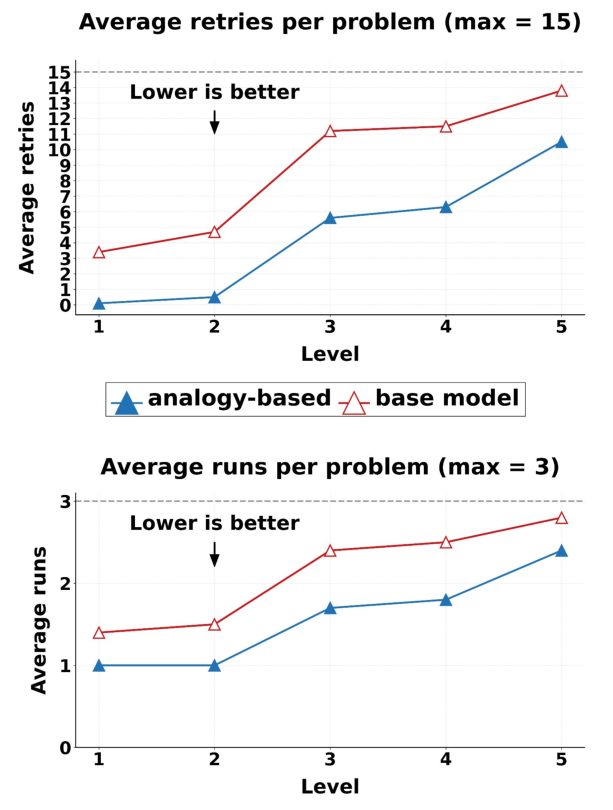
\includegraphics[width=0.39\textwidth]{latex/images/average_runs_retries.pdf}
\centering
\caption{
Average number of retries (top) and runs (bottom) per problem by difficulty level. The dashed line represents maximum allowed. Our analogy-based method consistently outperforms the base model (o1), with fewer retries and runs across all levels.
}
\label{fig:avg_runs_retries}
\end{figure}



\begin{figure}[t]
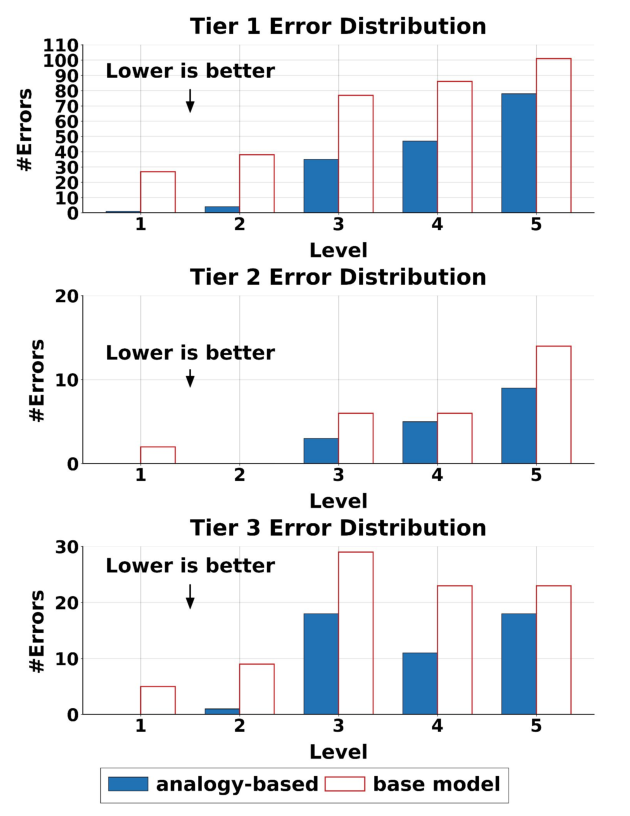
\includegraphics[width=0.39\textwidth]{latex/images/ErrorDist.pdf}
\centering
\caption{Error distribution by tier for our method vs. (o1) base model. Our method reduces errors across all tiers, with tier-1 errors being most frequent in both. }
\label{fig:error_dist}
\end{figure}


\noindent\textbf{Error analysis.}
As detailed in Section~\ref{subsec:verifier}, we categorize verifier errors into three tiers. Figure~\ref{fig:error_dist} shows their distribution across difficulty levels.
Our method yields fewer errors than the base model across all tiers and levels.
Tier-1 syntax errors are the most prevalent, followed by Tier-3 errors, where the proof fails to establish the goal. Tier-2 errors, involving theorem calls with violated premises, are the least common. This trend also holds for the base model.
Tier-1 errors are frequent but easily corrected with verifier feedback, whereas Tier-2 errors reflect deeper geometric reasoning failures that often persist across retries. Thus, verification removes superficial errors, leaving reasoning failures as the main performance bottleneck.






